\documentclass[10pt]{beamer}
\usetheme[
%%% option passed to the outer theme
%    progressstyle=fixedCircCnt,   % fixedCircCnt, movingCircCnt (moving is default)
  ]{Feather}

% If you want to change the colors of the various elements in the theme, edit and uncomment the following lines

% Change the bar colors:
%\setbeamercolor{Feather}{fg=red!20,bg=red}

% Change the color of the structural elements:
%\setbeamercolor{structure}{fg=red}

% Change the frame title text color:
%\setbeamercolor{frametitle}{fg=blue}

% Change the normal text color background:
%\setbeamercolor{normal text}{fg=black,bg=gray!10}

%-------------------------------------------------------
% INCLUDE PACKAGES
%-------------------------------------------------------

\usepackage[utf8]{inputenc}
\usepackage[english]{babel}
\usepackage[T1]{fontenc}
\usepackage{booktabs}
\usepackage{helvet}

\usepackage{amsthm}
\theoremstyle{definition}

%-------------------------------------------------------
% DEFINING AND REDEFINING COMMANDS
%-------------------------------------------------------

% colored hyperlinks
\newcommand{\chref}[2]{
  \href{#1}{{\usebeamercolor[bg]{Feather}#2}}
}

%-------------------------------------------------------
% DEFFINING AND REDEFINING CUSTOM COMMANDS
%-------------------------------------------------------
\newcommand{\Stitle}{Cayley's Formula for the Number of Trees: 2 Proofs}
\newcommand{\Stableofcontents}{Table of Contents}
\newcommand{\Sone}{Introduction}
\newcommand{\SoneSSdefinitions}{Definitions}
\newcommand{\SoneSSexamples}{Examples}
\newcommand{\SoneSSintuition}{Intuition}
\newcommand{\SoneSStheorem}{Theorem}
\newcommand{\Stwo}{Proof using Double Counting}
\newcommand{\StwoSSdefinitions}{Definitions}
\newcommand{\StwoSSstructure}{Proof Structure}
\newcommand{\StwoSSproof}{Proof}
\newcommand{\Sthree}{Proof using a Bijection}
\newcommand{\SthreeSSdefinitions}{Definitions}
\newcommand{\SthreeSSstructure}{Proof Structure}
\newcommand{\SthreeSSproof}{Proof}
\newcommand{\Sfour}{Conclusion}
\newcommand{\SfourSSreference}{References}

\newcommand{\DefColor}{purple}

%-------------------------------------------------------
% INFORMATION IN THE TITLE PAGE
%-------------------------------------------------------

\title[Cayley's Formula for the Number of Trees: 2 Proofs] % [] is optional - is placed on the bottom of the sidebar on every slide
{ % is placed on the title page
      \textbf{\Stitle}
}

\subtitle[\Stitle]
{
      \textbf{v. 1.0.0}
}

\author[Robert Lech]
{
      Robert Lech - {\ttfamily robert.lech@carleton.ca}
}

\institute[]
{
      Faculty of Mathematics,
      Carleton University\\

  %there must be an empty line above this line - otherwise some unwanted space is added between the university and the country (I do not know why;( )
}

\date{\today}

%-------------------------------------------------------
% THE BODY OF THE PRESENTATION
%-------------------------------------------------------

\begin{document}

%-------------------------------------------------------
% THE TITLEPAGE
%-------------------------------------------------------

{\1% % this is the name of the PDF file for the background
\begin{frame}[plain,noframenumbering] % the plain option removes the header from the title page, noframenumbering removes the numbering of this frame only
  \titlepage{} % call the title page information from above
\end{frame}}


\begin{frame}{\Stableofcontents}{}
\tableofcontents
\end{frame}

%-------------------------------------------------------
\section{\Sone}
%-------------------------------------------------------
\subsection{\SoneSSdefinitions}
\begin{frame}{\Sone}{\SoneSSdefinitions}
% Include some basic definitions
\begin{definition}
A \textbf{\textcolor{\DefColor}{graph}} is a tuple $G=(V, E)$ where $V$ is the set of \textbf{vertices} and $E$ is the set of \textbf{edges}, each with endpoints in $V$.
\end{definition}

\pause{}

\begin{definition}
A graph can have \textbf{\textcolor{\DefColor}{labelled vertices}}. We then denote $V=\{1, 2, \ldots,n\}$ for simplicity.
\end{definition}

\end{frame}

%-------------------------------------------------------
\begin{frame}{\Sone}{\SoneSSdefinitions}

\begin{definition}
A \textbf{\textcolor{\DefColor}{simple graph}} is a graph with \textbf{no loops or multiple edges}.
\end{definition}

\begin{figure}
  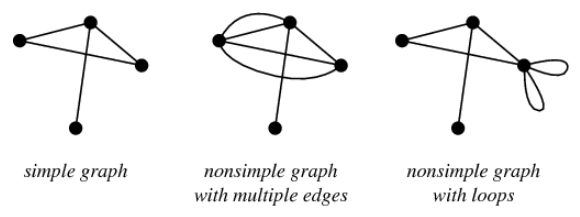
\includegraphics[width=\linewidth]{images/section1_simple.png}
  \caption{Simple vs.\ non-simple graph}
  \label{fig:section1_simple}
\end{figure}

\end{frame}

%-------------------------------------------------------
\begin{frame}{\Sone}{\SoneSSdefinitions}
% Include some basic definitions
\begin{definition}
Let $C=v_{0}e_{1}v_{1}e_{2}\ldots e_{k}v_{k}$ be an \textbf{alternating sequence of vertices and edges}. If $v_{0}, v_{1}, \ldots, v_{k-1}$ are distinct, $e_{1}, e_{2}, \ldots, e_{k}$ are distinct, and $v_{0}=v_{k}$, then $C$ is a \textbf{\textcolor{\DefColor}{cycle}}.
\end{definition}

\pause{}

\begin{definition}
Let $G$ be a graph with \textbf{no cycles}. Then we say the graph is \textbf{\textcolor{\DefColor}{acyclic}}.
\end{definition}

\end{frame}

%-------------------------------------------------------
\begin{frame}{\Sone}{\SoneSSdefinitions}
% Include some basic definitions
\begin{definition}
Let $G=(V,E)$ be a graph where $V=\{V_{1}, V_{2}, \ldots, V_{k}\}$ where for vertices $v_{i} \in V_{i},v_{j} \in V_{j}$ s.t. $i\neq j$, there \textbf{doesn't exists a path between $v_{i}$ and $v_{j}$}. Then we say $G$ has $k$ \textbf{\textcolor{\DefColor}{components}} or $c(G)=k$.
\end{definition}

\pause{}

\begin{definition}
An acyclic graph with \textbf{1 component} is called a \textbf{\textcolor{\DefColor}{tree}}.

An acyclic graph with \textbf{more than 1 component} is called a \textbf{\textcolor{\DefColor}{forest}}.
\end{definition}

\end{frame}

%-------------------------------------------------------
\subsection{\SoneSSexamples}
\begin{frame}{\Sone}{\SoneSSexamples}
% Examples of trees of size 1,2,3
\begin{figure}
  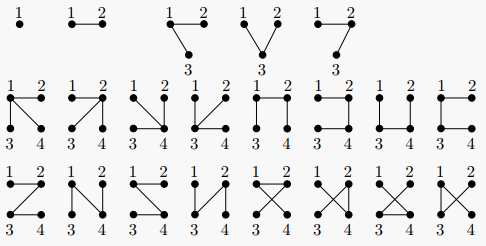
\includegraphics[width=\linewidth]{images/section1_trees_1_to_4.png}
  \caption{Labelled trees with $n=1,2,3,4$ vertices}
  \label{fig:trees_1_to_4}
\end{figure}

\end{frame}

%-------------------------------------------------------
\begin{frame}{\Sone}{\SoneSSintuition}
% Observation Table
\begin{block}{The Question}
How many labelled trees are there with $n$ vertices?
\end{block}

\pause{}

\begin{block}{Sample Values}
\begin{table}[ht]
\centering
\begin{tabular}[t]{cc}
\toprule
n&\# of labelled trees\\
\midrule
1&1   \\
2&1   \\
3&3   \\
4&6   \\
5&125 \\
\bottomrule
\label{tab:values}
\end{tabular}
\caption{Table showing number of labelled trees vs number of vertices}
\end{table}
\end{block}

\end{frame}
%-------------------------------------------------------

\begin{frame}{\Sone}{\SoneSSintuition}
% Observation Table
\begin{block}{The Question}
How many labelled trees are there with $n$ vertices?
\end{block}

\begin{block}{Sample Values}
\begin{table}[]
\centering
\begin{tabular}{ll}
\toprule
n & \# of labelled trees                   \\
\midrule
1 & 1   \textcolor{blue}{$(= 1^{1-2})$}    \\
2 & 1   \textcolor{blue}{$(= 2^{2-2})$}    \\
3 & 3   \textcolor{blue}{$(= 3^{3-2})$}    \\
4 & 16  \textcolor{blue}{$(= 4^{4-2})$}    \\
5 & 125 \textcolor{blue}{$(= 5^{5-2})$}    \\
\bottomrule
\end{tabular}
\caption{Table showing number of labelled trees vs number of vertices (showing the relationship)}
\label{tab:values-relationship}
\end{table}
\end{block}

\end{frame}

%-------------------------------------------------------
\subsection{\SoneSStheorem}
\begin{frame}{\Sone}{\SoneSStheorem}
% State the Theorem
\begin{block}{The Theorem}
The are $n^{n-2}$ labelled trees with $n$ vertices.
\end{block}

\pause{}

\begin{block}{Approach}
Prove this with two methods:
\begin{itemize}
  \item Double Counting
  \pause{}
  \item Finding a Bijection
\end{itemize}
\end{block}

\end{frame}

%-------------------------------------------------------
\section{\Stwo}
%-------------------------------------------------------
\subsection{\StwoSSdefinitions}
\begin{frame}{\Stwo}{\StwoSSdefinitions}
% State the necessary definitions
\begin{definition}
A \textbf{\textcolor{\DefColor}{directed graph}} (or digraph) is another form of a labelled tree where \textbf{edges point in a direction}.
\end{definition}

\pause{}

\begin{definition}
Let $G=(V,E)$ and $G'=(V',E')$ such that \textbf{$V'$ is a subset of $V$ and $E'$ is a subset of $E$} (and labels are preserved). Then $G'\subseteq G$ and we say $G'$ is a \textbf{\textcolor{\DefColor}{subgraph}} of $G$.
\end{definition}

\pause{}

\begin{definition}
A \textbf{\textcolor{\DefColor}{rooted forest}} is a forest where \textbf{every component has a distinguished vertex selected to be `the root'}.
\end{definition}

\end{frame}

%-------------------------------------------------------
\begin{frame}{\Stwo}{\StwoSSproof}
% Do the proof

\begin{figure}
  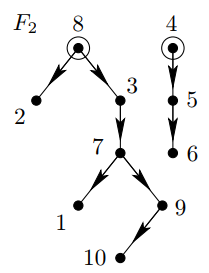
\includegraphics[width=0.4\linewidth]{images/section2_example.png}
  \caption{Example of a rooted forest with 2 components.}
  \label{fig:section2_example}
\end{figure}

\end{frame}

%-------------------------------------------------------
\subsection{\StwoSSstructure}
\begin{frame}{\Stwo}{\StwoSSstructure}
% Explain the proof structure
\begin{block}{Method}
Count the number of rooted trees of $n$ vertices in \textbf{two ways}
\begin{enumerate}
  \item count the number of ways to remove branches from a tree
  \pause{}
  \item count the number of ways to piece components of a forest together to create a tree
\end{enumerate}
\end{block}

\end{frame}

%-------------------------------------------------------
\subsection{\StwoSSproof}
\begin{frame}{\Stwo}{\StwoSSproof}
% Do the proof
\begin{block}{Fact}
Let $\mathcal{F}_{n,k}$ be the set of all rooted forests with $n$ vertices and $k$ components. Let $F_{n,k}$ be a directed forest with all edges facing away from the root vertex.

\textbf{Fact}: Let $F'\subseteq F$, both with $n$ vertices. Then $c(F')>c(F)$.

Note that each component $F$ is acyclic $\implies$ each edge is a cut edge $\implies$ $F$
\textbackslash{} $\{e\}$ splits a component in two.
\end{block}

\pause{}

\begin{block}{Define}
Let the sequence $F_{1},\ldots, F_{k}$ of forests be a refining sequence.
\begin{itemize}
  \item That is: $\forall i$, $F_{i+1}\subseteq F_{i}$.
\end{itemize}
\end{block}

\pause{}

\begin{block}{Define}
Denote $N(F_{k})$ to be the number of rooted trees containing $F_{k}$

Denote $N^{*}(F_{k})$ to be the number of refining sequences ending in $F_{k}$.
\end{block}

\end{frame}

%-------------------------------------------------------
\begin{frame}{\Stwo}{\StwoSSproof}
% Do the proof

\begin{block}{Approach}
We'll count this in two different ways. First, by starting at $F_{1}$ and working to $F_{k}$. The second way will be done backwards.
\end{block}

\pause{}

\begin{figure}
  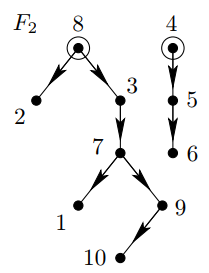
\includegraphics[width=0.3\linewidth]{images/section2_example.png}
  \caption{Example of a rooted forest with 2 components.}
  \label{fig:section2_example2}
\end{figure}

\end{frame}

%-------------------------------------------------------
\begin{frame}{\Stwo}{\StwoSSproof}

\begin{block}{Equation}
We note that for any subgraph $F_{k}$ of $F_{1}$, there are $(k-1)!$ ways remove % chktex 40
$(k-1)$ edges. Therefore, we have that:

\[
  N^{*}(F_{k})=N(F_{k})(k-1)!
\]
\end{block}

\begin{figure}
  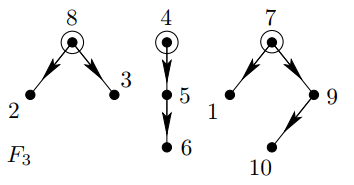
\includegraphics[width=0.6\linewidth]{images/section2_subgraph.png}
  \caption{Removing an edge from $F_{2}$ to create $F_{3}$}
  \label{fig:section2_subgraph}
\end{figure}

\end{frame}

%-------------------------------------------------------
\begin{frame}{\Stwo}{\StwoSSproof}

\begin{block}{Equation}
Going backwards, suppose we have $F_{k}$. Note that we have $n(k-1)$ ways to create $F_{k-1}$. We repeat this and get:

\[
  N^{*}(F_{k})=n(k-1)n(k-2)\ldots n(1)=n^{k-1}(k-1)!
\]
\end{block}

\begin{figure}
  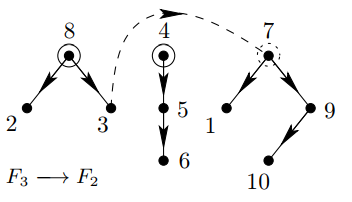
\includegraphics[width=0.55\linewidth]{images/section2_rejoin.png}
  \caption{Adding an edge to $F_{3}$ to create $F_{2}$}
  \label{fig:section2_rejoin}
\end{figure}

\end{frame}

%-------------------------------------------------------
\begin{frame}{\Stwo}{\StwoSSproof}

\begin{block}{Equation}
Giving us $N(F_{k})(k-1)!=n^{k-1}(k-1)!$ which implies: % chktex 40
\[
  N(F_{k})=n^{k-1}
\]
However $F_{n}$ is $n$ isolated vertices. So $N(F_{n})=n^{n-1}$ counts the number of all rooted trees (since all trees with $n$ vertices contains $n$ disjoint vertices as a subgraph) so we have the number of trees with $n$ vertices is $n^{n-2}$.
\end{block}

\end{frame}

%-------------------------------------------------------
\section{\Sthree}
%-------------------------------------------------------
\subsection{\SthreeSSstructure}
\begin{frame}{\Sthree}{\SthreeSSstructure}
% State the Theorem
\begin{block}{Introduction}
In this proof, we'll aim to uniquely encode every tree by a sequence $(a_{1},a_{2},\ldots a_{n-2})$. To do this, we look at a labelled tree on $N=\{1, 2, \ldots, n\}$. Moreover, suppose 2 (not-necessarily distinct) vertices are selected to have the $\bigcirc$ and $\square$ to denote the \textit{left vertex} and \textit{right vertex}. Let $\mathcal{T}_{n}=\{(t; \bigcirc, \square)\}$ be a new set. Note $|\mathcal{T}_{n}|=n^{2}T_{n}$.
\end{block}

\pause{}

\begin{figure}
  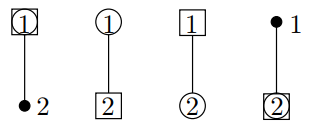
\includegraphics[width=0.6\linewidth]{images/section3_example.png}
  \caption{Example showing that the circle and square labels give us 4 times the number of trees.}
  \label{fig:section3_example}
\end{figure}

\end{frame}

%-------------------------------------------------------
\subsection{\SthreeSSproof}
\begin{frame}{\Sthree}{\SthreeSSproof}
% Prove the theorem
We want to show $|\mathcal{T}_{n}|=n^{n}$. Naturally, we'd like to there's a bijection between this set and the set of mappings from $N$ into $N$.

Let $f:N \rightarrow N$ be any map. We represent $f$ as a directed graph $\vec G_{f}$ by drawing arrows from $i$ to $f(i)$.

\end{frame}

%-------------------------------------------------------
\begin{frame}{\Sthree}{\SthreeSSproof}

For example, the map:

\[
  a = \left(\begin{matrix}
    1 & 2 & 3 & 4 & 5 & 6 & 7 & 8 & 9 & 10 \\
    7 & 5 & 5 & 9 & 1 & 2 & 5 & 8 & 4 & 7
  \end{matrix}\right)
\]

\pause{}

This is represented by the directed graph below:

\begin{figure}
  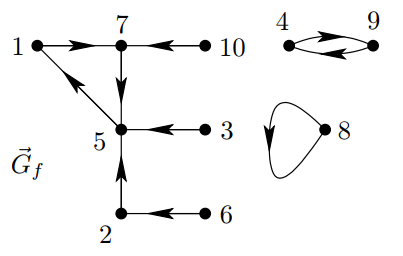
\includegraphics[width=0.6\linewidth]{images/section3_graph.png}
  \caption{The graph associated with map $f$}
  \label{fig:section3_graph}
\end{figure}

\end{frame}

%-------------------------------------------------------
\begin{frame}{\Sthree}{\SthreeSSproof}

Note:
\begin{itemize}
  \item one, and only one, edge emanating from each vertex
  \item implies one, and only one, cycle per component
\end{itemize}

\pause{}

Let $M=\{a_{1}, a_{2}, \ldots, a_{l}\} \subseteq N$ be the union of the vertex sets of these cycles such that they are sorted in increasing order.

\[
  f|_{M} = \left(\begin{matrix}
      a_{1}  &   a_{2}  & \cdots &   a_{l} \\
    f(a_{1}) & f(a_{2}) & \cdots & f(a_{l})
  \end{matrix}\right)
\]

In our example, we have:

\[
  f|_{M} = \left(\begin{matrix}
      1 & 4 & 5 & 7 & 8 & 9 \\
      7 & 9 & 1 & 5 & 8 & 4
  \end{matrix}\right)
\]

\end{frame}

%-------------------------------------------------------
\begin{frame}{\Sthree}{\SthreeSSproof}
Note:
\begin{itemize}
  \item In the second row, we have $f(a_{1}), f(a_{2}), \ldots, f(a_{l})$ in a specific order.
  \pause{}
  \item Let $\bigcirc=f(a_{1})$ and $\square=f(a_{l})$.
  \pause{}
  \item Create a $(f(a_{1}),f(a_{l}))$-path such that each vertex in $M$ acts as its own root with all incoming vertices dangling from that root.
\end{itemize}

\pause{}

\begin{figure}
  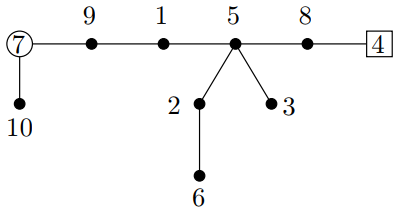
\includegraphics[width=0.6\linewidth]{images/section3_tree.png}
  \caption{The tree associated with map $f|_{M}$}
  \label{fig:section3_tree}
\end{figure}

\end{frame}

%-------------------------------------------------------
\begin{frame}{\Sthree}{\SthreeSSproof}
% Conclude the proof by stating the reverse process is determined uniquely
\begin{enumerate}
  \item Given a tree and vertex pair $\{(t; \bigcirc, \square)\}$\ldots
  \pause{}
  \item Look at the unique path from $\bigcirc$ to $\square$\ldots
  \pause{}
  \item Create the mapping $f|_{M}$
  \pause{}
  \item Create the directed graph $\vec G_{f}$ from $f|_{M}$ and dangling branches $t$
  \pause{}
  \item Create the mapping $f$. This mapping is your encoding of the $\{(t; \bigcirc, \square)\}$
\end{enumerate}

\pause{}

A bijection from $\{(t; \bigcirc, \square)\} \rightarrow (a_{1},a_{2},\ldots a_{n})$ implies a bijection A bijection from $t \rightarrow (a_{1},a_{2},\ldots a_{n-2})$ -- and so we're done.

\end{frame}

%-------------------------------------------------------
\section{\Sfour}
%-------------------------------------------------------
\subsection{\SfourSSreference}
\begin{frame}{\Sfour}{\SfourSSreference}
% show references
\begin{block}{\SfourSSreference}
\begin{thebibliography}{9}
\bibitem{latexcompanion}
Aigner, Martin, and Ziegler Gunter M.
\textit{Proofs from the book}.
5th ed., Springer, 2014.
\end{thebibliography}
\end{block}

\end{frame}

%-------------------------------------------------------
\end{document}
